\documentclass[11pt,preprint, authoryear]{elsarticle}

\usepackage{lmodern}
%%%% My spacing
\usepackage{setspace}
\setstretch{1.2}
\DeclareMathSizes{12}{14}{10}{10}

% Wrap around which gives all figures included the [H] command, or places it "here". This can be tedious to code in Rmarkdown.
\usepackage{float}
\let\origfigure\figure
\let\endorigfigure\endfigure
\renewenvironment{figure}[1][2] {
    \expandafter\origfigure\expandafter[H]
} {
    \endorigfigure
}

\let\origtable\table
\let\endorigtable\endtable
\renewenvironment{table}[1][2] {
    \expandafter\origtable\expandafter[H]
} {
    \endorigtable
}


\usepackage{ifxetex,ifluatex}
\usepackage{fixltx2e} % provides \textsubscript
\ifnum 0\ifxetex 1\fi\ifluatex 1\fi=0 % if pdftex
  \usepackage[T1]{fontenc}
  \usepackage[utf8]{inputenc}
\else % if luatex or xelatex
  \ifxetex
    \usepackage{mathspec}
    \usepackage{xltxtra,xunicode}
  \else
    \usepackage{fontspec}
  \fi
  \defaultfontfeatures{Mapping=tex-text,Scale=MatchLowercase}
  \newcommand{\euro}{€}
\fi

\usepackage{amssymb, amsmath, amsthm, amsfonts}

\def\bibsection{\section*{References}} %%% Make "References" appear before bibliography


\usepackage[round]{natbib}

\usepackage{longtable}
\usepackage[margin=2.3cm,bottom=2cm,top=2.5cm, includefoot]{geometry}
\usepackage{fancyhdr}
\usepackage[bottom, hang, flushmargin]{footmisc}
\usepackage{graphicx}
\numberwithin{equation}{section}
\numberwithin{figure}{section}
\numberwithin{table}{section}
\setlength{\parindent}{0cm}
\setlength{\parskip}{1.3ex plus 0.5ex minus 0.3ex}
\usepackage{textcomp}
\renewcommand{\headrulewidth}{0pt}
\renewcommand{\footrulewidth}{0.3pt}

\usepackage{array}
\newcolumntype{x}[1]{>{\centering\arraybackslash\hspace{0pt}}p{#1}}

%%%%  Remove the "preprint submitted to" part. Don't worry about this either, it just looks better without it:
\makeatletter
\def\ps@pprintTitle{%
  \let\@oddhead\@empty
  \let\@evenhead\@empty
  \let\@oddfoot\@empty
  \let\@evenfoot\@oddfoot
}
\makeatother

 \def\tightlist{} % This allows for subbullets!

\usepackage{hyperref}
\hypersetup{breaklinks=true,
            bookmarks=true,
            colorlinks=true,
            citecolor=blue,
            urlcolor=blue,
            linkcolor=blue,
            pdfborder={0 0 0}}


% The following packages allow huxtable to work:
\usepackage{siunitx}
\usepackage{multirow}
\usepackage{hhline}
\usepackage{calc}
\usepackage{tabularx}
\usepackage{booktabs}
\usepackage{caption}


\newenvironment{columns}[1][]{}{}

\newenvironment{column}[1]{\begin{minipage}{#1}\ignorespaces}{%
\end{minipage}
\ifhmode\unskip\fi
\aftergroup\useignorespacesandallpars}

\def\useignorespacesandallpars#1\ignorespaces\fi{%
#1\fi\ignorespacesandallpars}

\makeatletter
\def\ignorespacesandallpars{%
  \@ifnextchar\par
    {\expandafter\ignorespacesandallpars\@gobble}%
    {}%
}
\makeatother

\newlength{\cslhangindent}
\setlength{\cslhangindent}{1.5em}
\newenvironment{CSLReferences}%
  {\setlength{\parindent}{0pt}%
  \everypar{\setlength{\hangindent}{\cslhangindent}}\ignorespaces}%
  {\par}


\urlstyle{same}  % don't use monospace font for urls
\setlength{\parindent}{0pt}
\setlength{\parskip}{6pt plus 2pt minus 1pt}
\setlength{\emergencystretch}{3em}  % prevent overfull lines
\setcounter{secnumdepth}{5}

%%% Use protect on footnotes to avoid problems with footnotes in titles
\let\rmarkdownfootnote\footnote%
\def\footnote{\protect\rmarkdownfootnote}
\IfFileExists{upquote.sty}{\usepackage{upquote}}{}

%%% Include extra packages specified by user
\usepackage{booktabs}
\usepackage{longtable}
\usepackage{array}
\usepackage{multirow}
\usepackage{wrapfig}
\usepackage{float}
\usepackage{colortbl}
\usepackage{pdflscape}
\usepackage{tabu}
\usepackage{threeparttable}
\usepackage{threeparttablex}
\usepackage[normalem]{ulem}
\usepackage{makecell}
\usepackage{xcolor}

%%% Hard setting column skips for reports - this ensures greater consistency and control over the length settings in the document.
%% page layout
%% paragraphs
\setlength{\baselineskip}{12pt plus 0pt minus 0pt}
\setlength{\parskip}{12pt plus 0pt minus 0pt}
\setlength{\parindent}{0pt plus 0pt minus 0pt}
%% floats
\setlength{\floatsep}{12pt plus 0 pt minus 0pt}
\setlength{\textfloatsep}{20pt plus 0pt minus 0pt}
\setlength{\intextsep}{14pt plus 0pt minus 0pt}
\setlength{\dbltextfloatsep}{20pt plus 0pt minus 0pt}
\setlength{\dblfloatsep}{14pt plus 0pt minus 0pt}
%% maths
\setlength{\abovedisplayskip}{12pt plus 0pt minus 0pt}
\setlength{\belowdisplayskip}{12pt plus 0pt minus 0pt}
%% lists
\setlength{\topsep}{10pt plus 0pt minus 0pt}
\setlength{\partopsep}{3pt plus 0pt minus 0pt}
\setlength{\itemsep}{5pt plus 0pt minus 0pt}
\setlength{\labelsep}{8mm plus 0mm minus 0mm}
\setlength{\parsep}{\the\parskip}
\setlength{\listparindent}{\the\parindent}
%% verbatim
\setlength{\fboxsep}{5pt plus 0pt minus 0pt}



\begin{document}



\begin{frontmatter}  %

\title{Covariance Matrix Estimation via Macroeconomic Factor Modeling}

% Set to FALSE if wanting to remove title (for submission)




\author[Add1]{Tiago Baltazar (19776209)}
\ead{tiagobaltazar15@gmail.com}





\address[Add1]{Stellenbosch University, Western Cape, South Africa}


\begin{abstract}
\small{
This report compares the performance of two asset allocation strategies
namely; Risk Parity and Mean Variance during periods of volatility in
South Africa. Using South African financial data, the risk adjusted and
information ratio of a unleverd Risk Parity Index porfolio and Tangency
Index porfolio are compared. The research paper found that the Mean
Variance Optimisation approach is an superior asset allocation strategy
during periods of high volatility in South Africa.
}
\end{abstract}

\vspace{1cm}


\begin{keyword}
\footnotesize{
Factor Modeling \sep Macroeconomic Factors \sep Asset Returns
\sep Covariance Matrix \\
\vspace{0.3cm}
}
\end{keyword}



\vspace{0.5cm}

\end{frontmatter}



%________________________
% Header and Footers
%%%%%%%%%%%%%%%%%%%%%%%%%%%%%%%%%
\pagestyle{fancy}
\chead{}
\rhead{19776209}
\lfoot{}
\rfoot{\footnotesize Page \thepage}
\lhead{\leftmark}
%\rfoot{\footnotesize Page \thepage } % "e.g. Page 2"
\cfoot{}

%\setlength\headheight{30pt}
%%%%%%%%%%%%%%%%%%%%%%%%%%%%%%%%%
%________________________

\headsep 35pt % So that header does not go over title




\hypertarget{introduction}{%
\section{\texorpdfstring{Introduction
\label{Intro}}{Introduction }}\label{introduction}}

Macroeconomic factor models use observable economic time series to
explain the common variation in asset returns, with the unexplained,
idiosyncratic, variance being asset-specific.

Overall investment risk is typically classified as being either
systematic (market), affecting the broader market, or idiosyncratic
risk, which is unique to individual assets. While the latter can, in
effect, be diversified away, the former affects a large portion of
assets. Factor models can be used to explain the common (systematic)
variation in asset returns, with the remaining variance, not explained
by the factors, being unique to each individual security.

\hypertarget{literature-review}{%
\section{\texorpdfstring{Literature Review
\label{Lit}}{Literature Review }}\label{literature-review}}

The use of modern, multivariate, factor models can be seen as an
extension of the seminal work of
\protect\hyperlink{ref-Sharpe1964}{Sharpe}
(\protect\hyperlink{ref-Sharpe1964}{1964})'s Capital Asset Pricing Model
(CAPM), which used a single factor- the market portfolio- to estimate
asset returns. In most cases, however, there are potentially,
infinitely, many factors which can influence asset returns. Modern
factor models allow one to address the curse of dimensionality by
assuming stock returns are driven by a, more, limited set of factors.
Factor models thus decompose asset returns into two components: one
driven by the common variation between stocks, due to the factors, and
another idiosyncratic component, unique to each asset. Using a factor
model can therefore be a useful way of reducing the number of possible
parameters which can, possibly, drive asset returns; assuming that what
is not explained by the, common, factors is idiosyncratic risk unique to
each asset.

Factor models have gained in prominence since
\protect\hyperlink{ref-Sharpe1964}{Sharpe}
(\protect\hyperlink{ref-Sharpe1964}{1964}), and have been extended to
include more than one factor. In particular, this class of models can
generally be split into three types
(\protect\hyperlink{ref-Connor}{Connor, 1995}); macroeconomic,
statistical, and fundamental factor models. Whilst statistical factor
models use only the input (data) to determine the relevant factors for
asset returns, macroeceonmic and fundamental factor models rely on the
researcher to supplement the asset returns data with factors. One of the
most prominent fundamental factor model was developed by
\protect\hyperlink{ref-Fama1992}{Fama \& French}
(\protect\hyperlink{ref-Fama1992}{1992}), who use firm-specific
variables including relevant firm financial ratios, firm-size, and
market beta in order to explain the variation in asset returns.

In using macroeconomic factor models to study the behavior of asset
returns, \protect\hyperlink{ref-Chen1986}{Chen, Roll \& Ross}
(\protect\hyperlink{ref-Chen1986}{1986}) propose a set of candidate
economic variables as factors to explain systematic asset risk. They
found that industrial production, changes in risk premium, some measures
of inflation, and changes in the yield curve were all significant in
explaining expected asset returns. In a similar vein,
\protect\hyperlink{ref-Kim1987}{Kim \& Wu}
(\protect\hyperlink{ref-Kim1987}{1987}) find that an economic factor
model, generally, performs better than a multivariate CAPM. The factors
that they found to be significant were split into three categories:
general, economy-wide, variables, the second category focused on the
monetary side of the economy and included the interest rate and money
supply. And the final factor comprised of labor market variables.

\hypertarget{exploratory-analysis}{%
\section{\texorpdfstring{Exploratory Analysis
\label{Explor}}{Exploratory Analysis }}\label{exploratory-analysis}}

This section aims to provide a, brief, exploration of the data,
justifying the choice of macroeconomic variables used as factors, as
well as the treatment of the relevant assets.

\hypertarget{data-and-descriptive-statistics}{%
\subsection{Data and Descriptive
Statistics}\label{data-and-descriptive-statistics}}

\begin{table}[H]

\caption{\label{tab:Factors Description}Macroeconomic Factors}
\centering
\begin{tabular}[t]{l|l|l}
\hline
Name & Description & Source\\
\hline
Bcom\_Index & Bloomberg Commodities Index & N. Katzke\\
\hline
Inflation & Inflation (Consumer Prices) & IMF International Financial Statistics\\
\hline
MM.Rate & SA Money Market Rate & IMF International Financial Statistics\\
\hline
Real.GDP & SA Real Gross Domestic Product & IMF International Financial Statistics\\
\hline
Real.INV & SA Real Gross Fixed Capital Formation & IMF International Financial Statistics\\
\hline
US\_10Yr & US Long-Term Bond Yields & N. Katzke\\
\hline
USDZAR & USD/ZAR Spot Price & N. Katzke\\
\hline
VIX & CBOE Volatility Index & N. Katzke\\
\hline
\end{tabular}
\end{table}

\begin{longtable}[t]{l|l|l|l|l|l|l|l|l}
\caption{\label{tab:Descriptive Stats}Summary Statistics: Macroeconomic Factors}\\
\hline
  & US\_10Yr & Bcom\_Index & VIX & USDZAR & MM.Rate & Real.GDP & Real.INV & Inflation\\
\hline
median & 1.250 & 0.003 & -0.027 & 0.003 & 2.019 & 0.009 & 0.011 & 0.805\\
\hline
mean & 1.274 & -0.005 & 0.008 & 0.013 & 1.988 & 0.004 & 0.003 & 0.786\\
\hline
SE.mean & 0.038 & 0.012 & 0.040 & 0.008 & 0.029 & 0.004 & 0.005 & 0.038\\
\hline
CI.mean.0.95 & 0.077 & 0.024 & 0.080 & 0.017 & 0.058 & 0.007 & 0.011 & 0.076\\
\hline
var & 0.098 & 0.010 & 0.107 & 0.005 & 0.058 & 0.001 & 0.002 & 0.096\\
\hline
std.dev & 0.314 & 0.099 & 0.326 & 0.069 & 0.240 & 0.030 & 0.044 & 0.310\\
\hline
coef.var & 0.246 & -18.243 & 41.716 & 5.248 & 0.121 & 6.827 & 13.362 & 0.394\\
\hline
\end{longtable}

Tables 3.1 and 3.2, respectively, provide a description of the factors
included along with their sources, and summary statistics for the
factors. Macroeconomic factors for South Africa were chosen on the basis
of their possible influence in driving asset returns in South Africa. US
10 Year bond yields were used to quantify the influence of US Monetary
Policy decisions in driving global liquidity. This is based on the
direct relationship between bond yields and interest rates, whereby
lower interest rates depress bond yields and these thus become a less
attractive investment option; potentially leading investors to seek
higher returns in domestic and foreign asset markets. The Bloomberg
commodities index was used to measure the influence that changing
commodity prices may have on asset returns, given that the South African
economy is still influenced to a large extent by fluctuating commodity
prices. The CBOE VIX volatility index was included to account for the
effect that changing risk perceptions may have on domestic asset
returns. Similarly to changes in US long term bond yields, lower risk
perceptions may lead to capital flowing more towards developing
(periphery) and could thus influence South African asset returns. The
USDZAR spot rate was also included as changes in the price of foreign
exchange can influence asset returns through, for example, increasing
the cost of financing outstanding debt, or increasing input costs. The
money market rate was used to represent the domestic monetary policy
stance, this can affect the cost of borrowing for businesses, as well as
changing investor incentives when it comes to investing in asset
markets; both of which can influence returns. Real gross fixed capital
formation was used to account for the level of investment in the economy
for any given quarter. Finally, inflation was measured using the
quarterly growth in the Consumer Price Index (CPI).

\begin{table}[H]

\caption{\label{tab:T40 constituents}T40 Constituents: Financials}
\centering
\begin{tabular}[t]{l|l}
\hline
Ticker & Constituent\\
\hline
ABG & ABSA GROUP LTD\\
\hline
CPI & CAPITEC BANK HOL\\
\hline
DSY & DISCOVERY LTD\\
\hline
FSR & FIRSTRAND LTD\\
\hline
GRT & GROWTHPOINT PROP\\
\hline
INL & INVESTEC LTD\\
\hline
INP & INVESTEC PLC\\
\hline
NED & NEDBANK GROUP\\
\hline
NRP & NEPI ROCKCASTLE\\
\hline
OMU & OLD MUTUAL LTD\\
\hline
RNI & Reinet Investments SCA\\
\hline
SLM & SANLAM LTD\\
\hline
SBK & STANDARD BANK GR\\
\hline
\end{tabular}
\end{table}

\begin{table}[H]

\caption{\label{tab:unnamed-chunk-1}T40 Constituents: Industrials}
\centering
\begin{tabular}[t]{l|l}
\hline
Ticker & Constituent\\
\hline
APN & ASPEN PHARMACARE\\
\hline
BID & BID CORP LTD\\
\hline
BVT & BIDVEST GROUP\\
\hline
BTI & BRIT AMER TOBACC\\
\hline
CLS & CLICKS GROUP LTD\\
\hline
MNP & MONDI PLC\\
\hline
MRP & MR PRICE GROUP\\
\hline
MTN & MTN GROUP LTD\\
\hline
MCG & MULTICHOICE GROU\\
\hline
NPN & NASPERS LTD-N\\
\hline
PRX & PROSUS NV\\
\hline
CFR & RICHEMONT-DR\\
\hline
SHP & SHOPRITE HLDGS\\
\hline
SPP & SPAR GRP LTD/THE\\
\hline
VOD & VODACOM GROUP\\
\hline
WHL & WOOLWORTHS HLDGS\\
\hline
\end{tabular}
\end{table}

\begin{table}[H]

\caption{\label{tab:unnamed-chunk-2}T40 Constituents: Resources}
\centering
\begin{tabular}[t]{l|l}
\hline
Ticker & Constituent\\
\hline
AGL & ANGLO AMER PLC\\
\hline
AMS & ANGLO AMERICAN P\\
\hline
ANG & ANGLOGOLD ASHANT\\
\hline
BHP & BHP GROUP PLC\\
\hline
EXX & EXXARO RESOURCES\\
\hline
GLN & GLENCORE PLC\\
\hline
GFI & GOLD FIELDS LTD\\
\hline
IMP & IMPALA PLATINUM\\
\hline
NPH & NORTHAM PLATINUM\\
\hline
SOL & SASOL LTD\\
\hline
SSW & SIBANYE STILLWAT\\
\hline
\end{tabular}
\end{table}

For this analysis, only variables in the Top 40 stocks in the JSE with
the highest market capitalization were included. This was done to
account for the fact that larger companies will be more exposed to
global macroeconomic factors, relative to those with smaller market
caps. The variables chosen as part of this ``T40'' are based on the FTSE
Russell classification, as of the end of 2021 Q3 (see
(\protect\hyperlink{ref-FTSE}{{``Factsheet (ZAR) FTSE/JSE top 40
index''}, n.d.})). After subsetting the Top 40 stocks, these were
stratified into their respective super-industries. The stocks included,
as well as their relevant industries, can be found in Tables 3.3-3.5
above. In order to estimate the covariance matrix, there could be no
missing values in the asset returns data. Firstly, only those securities
which had more than 70\% of observations were considered, this led to
five assets dropping out: NRP, OMU, RNI, MCG, and PRX. The former three
were in financials, while the latter two were classified as industrials.
And secondly, returns were imputed according to their own probability
distribution. After this, there were no more missing values in the asset
returns data.

\hypertarget{data-visualization}{%
\subsection{Data Visualization}\label{data-visualization}}

This section presents figures for the relevant macroeconomic factors,
and the asset returns (disaggregated) by industry. All macro factors
entered the model in log terms, and, in addition, non-stationary
variables were taken as quarterly changes.

\begin{figure}[H]
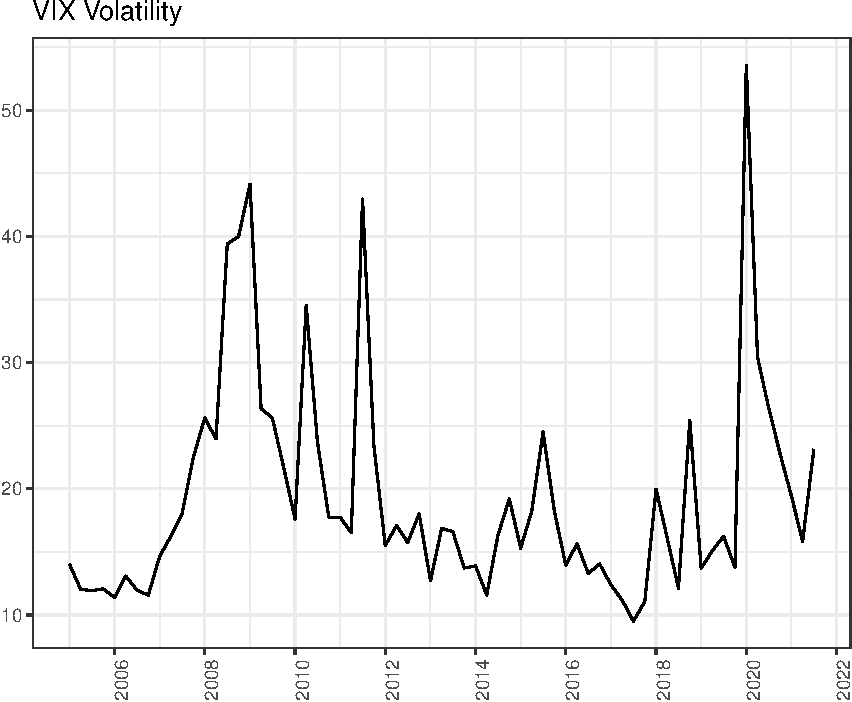
\includegraphics{Factor-Model_files/figure-latex/unnamed-chunk-3-1} \caption{US Long-Term Bond Yields \label{Fig1}}\label{fig:unnamed-chunk-3}
\end{figure}

\begin{figure}[H]
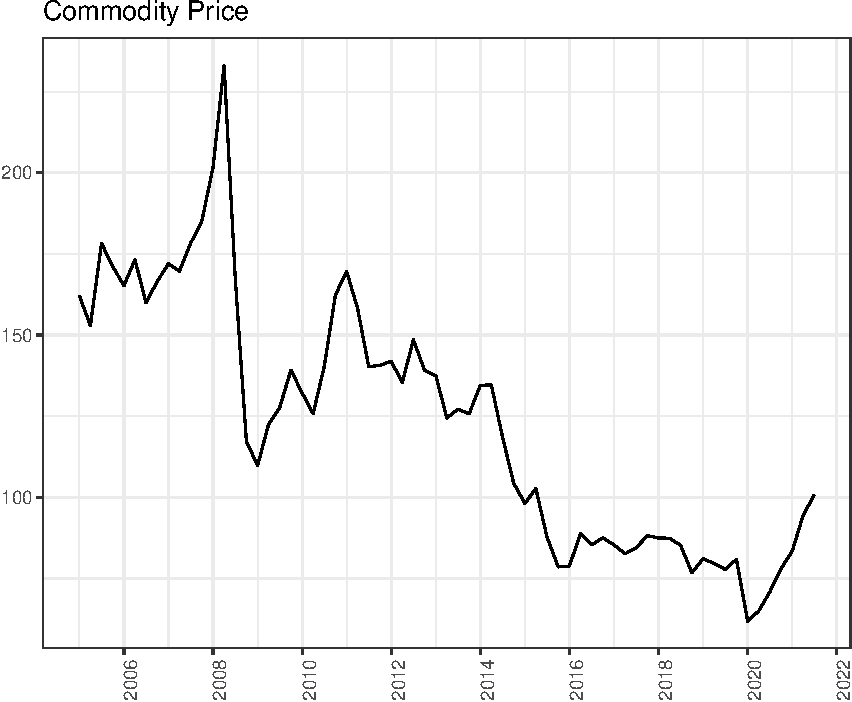
\includegraphics{Factor-Model_files/figure-latex/unnamed-chunk-4-1} \caption{USDZAR Spot Price \label{Fig2}}\label{fig:unnamed-chunk-4}
\end{figure}

\begin{figure}[H]
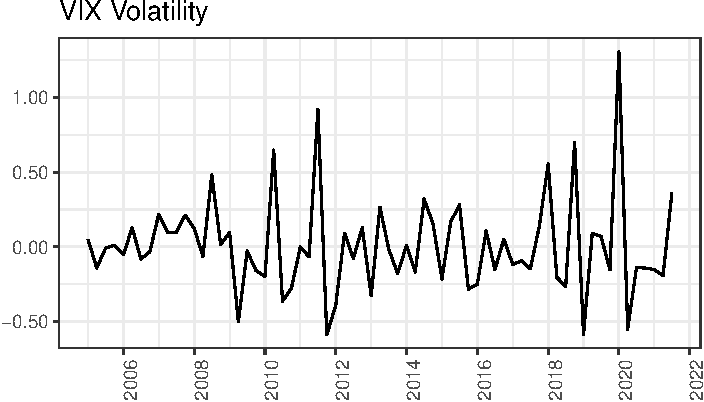
\includegraphics{Factor-Model_files/figure-latex/unnamed-chunk-5-1} \caption{CBOE VIX Volatility Index \label{Fig3}}\label{fig:unnamed-chunk-5}
\end{figure}

\begin{figure}[H]
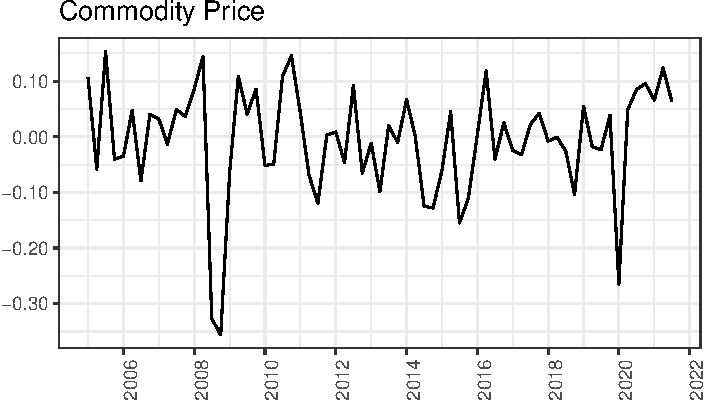
\includegraphics{Factor-Model_files/figure-latex/unnamed-chunk-6-1} \caption{Bloomberg Commodity Price Index \label{Fig4}}\label{fig:unnamed-chunk-6}
\end{figure}

\begin{figure}[H]
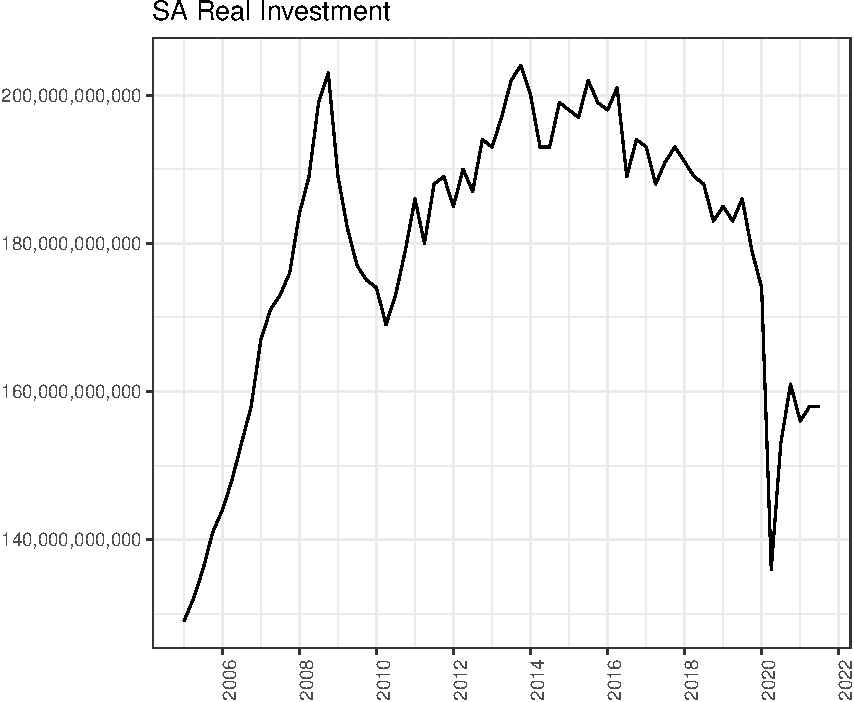
\includegraphics{Factor-Model_files/figure-latex/unnamed-chunk-7-1} \caption{South Africa Money Market Rate \label{Fig5}}\label{fig:unnamed-chunk-7}
\end{figure}

\begin{figure}[H]
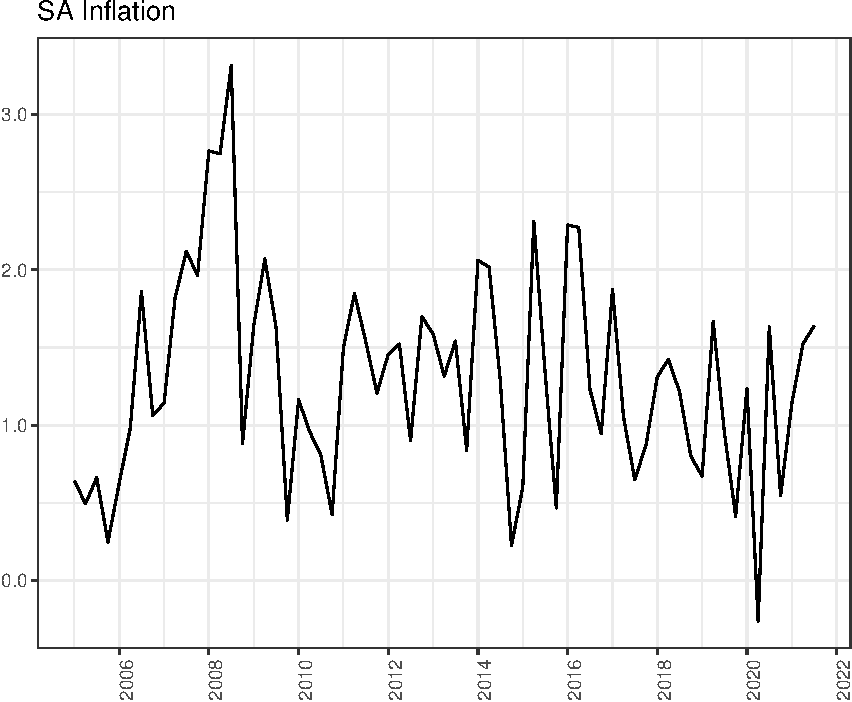
\includegraphics{Factor-Model_files/figure-latex/unnamed-chunk-8-1} \caption{South Africa Real GDP \label{Fig6}}\label{fig:unnamed-chunk-8}
\end{figure}

\begin{figure}[H]
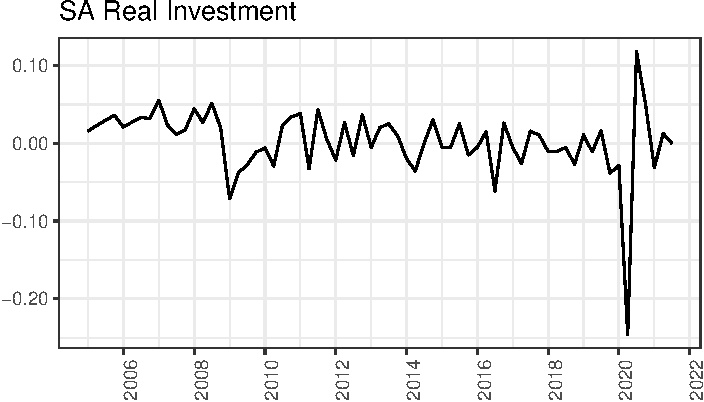
\includegraphics{Factor-Model_files/figure-latex/unnamed-chunk-9-1} \caption{South Africa Real Gross Fixed Capital Formation \label{Fig7}}\label{fig:unnamed-chunk-9}
\end{figure}

\begin{figure}[H]
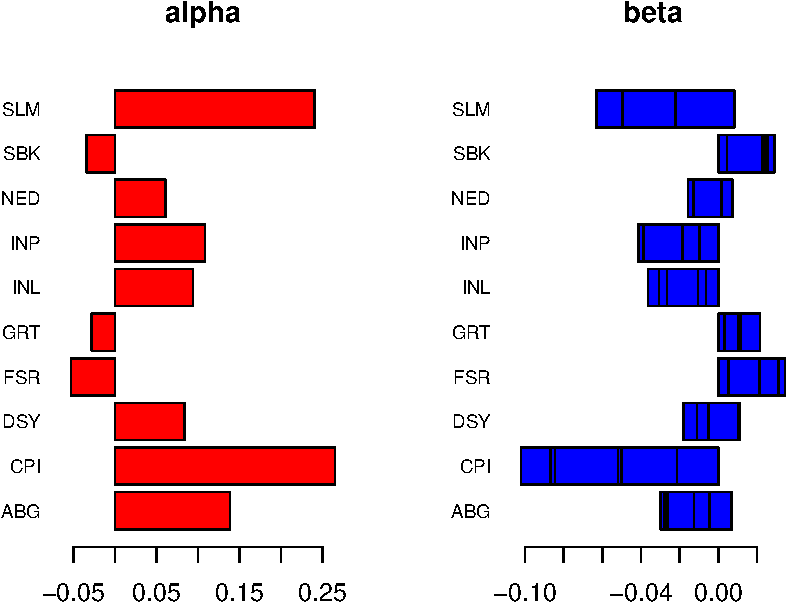
\includegraphics{Factor-Model_files/figure-latex/unnamed-chunk-10-1} \caption{South Africa Consumer Price Inflation \label{Fig8}}\label{fig:unnamed-chunk-10}
\end{figure}

\begin{figure}[H]
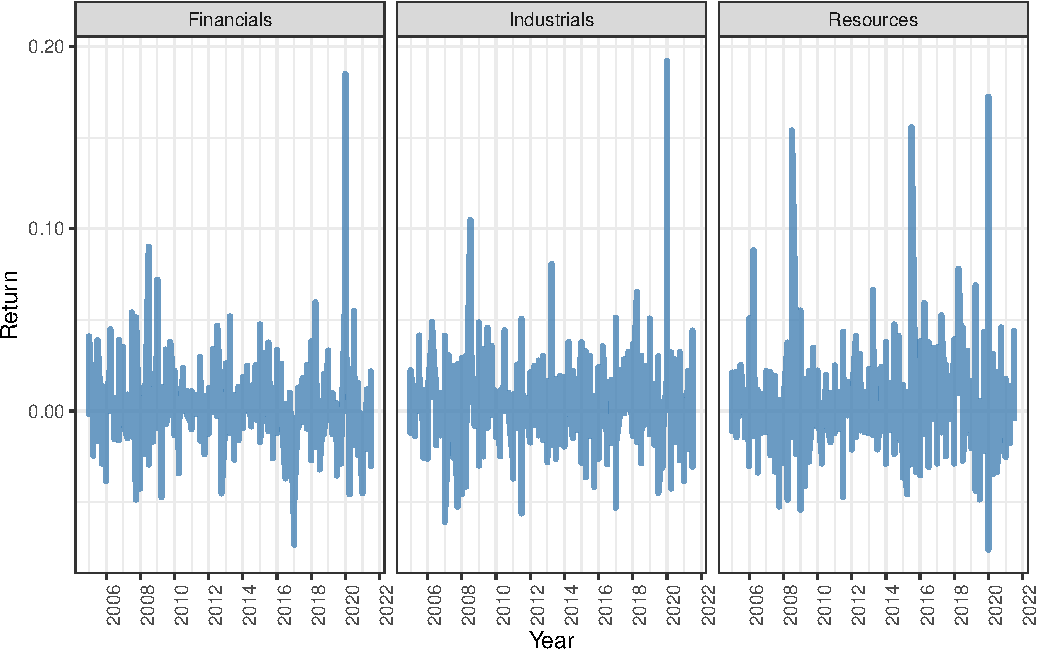
\includegraphics{Factor-Model_files/figure-latex/unnamed-chunk-11-1} \caption{Asset Returns by Industry \label{Fig9}}\label{fig:unnamed-chunk-11}
\end{figure}

\hypertarget{empirical-analysis}{%
\section{Empirical Analysis}\label{empirical-analysis}}

The model used to estimate covariance matrix parameters comprises of 8
macroeconomic factors, and 35 assets, disaggregated into their
respective super-industries. The macroeconomic factor model was then
applied to the three different industries, as these factors may affect
assets in different industries differently. These three industry classes
comprise of 10, 14, and 11 observations for the financial, industrial,
and resources sectors, respectively. This section presents the main
contribution of this paper, and the rest of it is set up as follows.
Section \ref{Meth} presents the methodology used when constructing the
macroeconomic factor model, Section \ref{Est} presents the results from
estimating the model, and finally, Section \ref{Disc} provides a
discussion of the main results.

\hypertarget{methodology}{%
\subsection{\texorpdfstring{Methodology
\label{Meth}}{Methodology }}\label{methodology}}

The equation of the model is given by:

\begin{align}
R_{ji,t}=\alpha_{ji} + \beta_{ji1}F_{1t} + ... + \beta_{jik}F_{kt} +...+\beta_{jiK}F_{Kt} +\epsilon_{it}
\end{align}

With \textbf{\(F\)} representing the 8 factors included in estimation,
\(\beta_{ik}\) representing the sensitivity of asset \(i\) to factor
\(k\), \((k=1,...,K)\), for industry \(j=(F,I,R)\). Factor models rely
on three main assumptions. Firstly, individual factor realizations have
zero expected value: \(\mathbb{E}(f_k)=0\). Secondly, asset-specific
errors are uncorrelated with each of the factors:
\(cov(f_{kt}, \epsilon_{it})=0\) \(\forall\) \(k\), \(i\), \& \(t\).
And, finally, that error terms are serially uncorrelated:
\(cov(\epsilon_{it}, \epsilon{ds})=0\) \(\forall\) \(i\neq d\), and
\(t \neq s\). From this, one then essentially has that:

\begin{align}
Var(r_{i}) = L\phi L' + \sigma
\end{align}

With the above implying that the variance of individual assets is given
by the sum of both the systematic and idiosyncratic risk components.

\hypertarget{model-estimation}{%
\subsection{\texorpdfstring{Model Estimation
\label{Est}}{Model Estimation }}\label{model-estimation}}

This section presents the results from estimating the macroeconomic
factor model, with \ref{Fig10}-\ref{Fig12} displaying the estimated
\textbf{\(\alpha\)'s} and \textbf{\(\beta\)'s} for each industry, where
\(\beta\) represents each assets sensitivity to the factors, and alpha
the constant (excess) returns.

\begin{figure}[H]
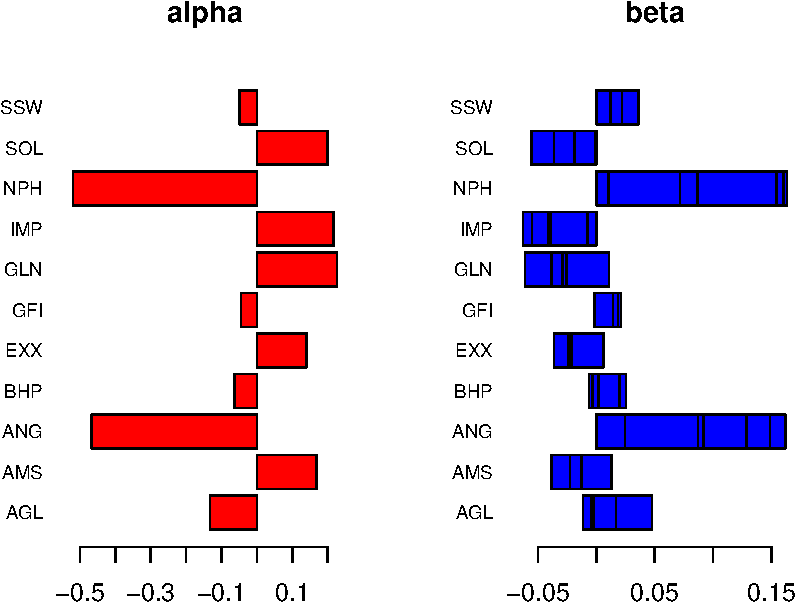
\includegraphics{Factor-Model_files/figure-latex/unnamed-chunk-12-1} \caption{Factor Analysis: Financials \label{Fig10}}\label{fig:unnamed-chunk-12}
\end{figure}

\begin{figure}[H]
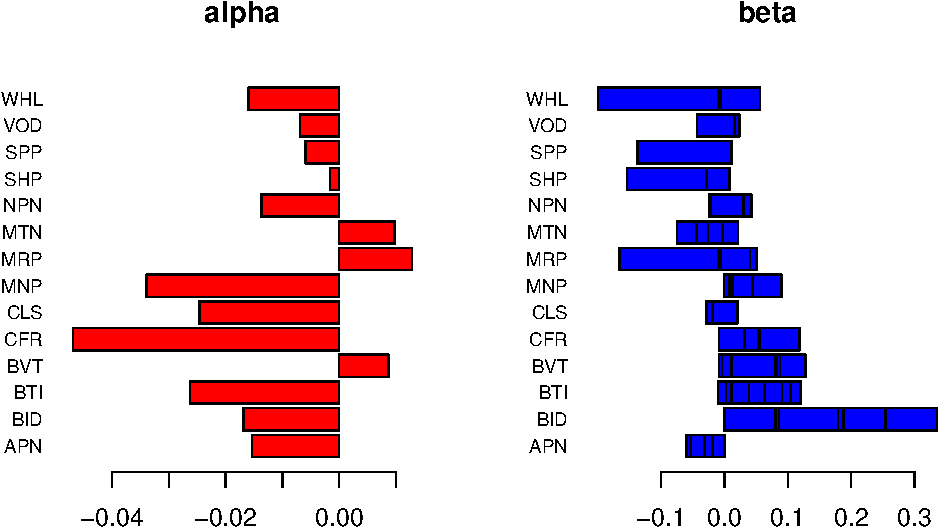
\includegraphics{Factor-Model_files/figure-latex/unnamed-chunk-13-1} \caption{Factor Analysis: Industrial \label{Fig11}}\label{fig:unnamed-chunk-13}
\end{figure}

\begin{figure}[H]
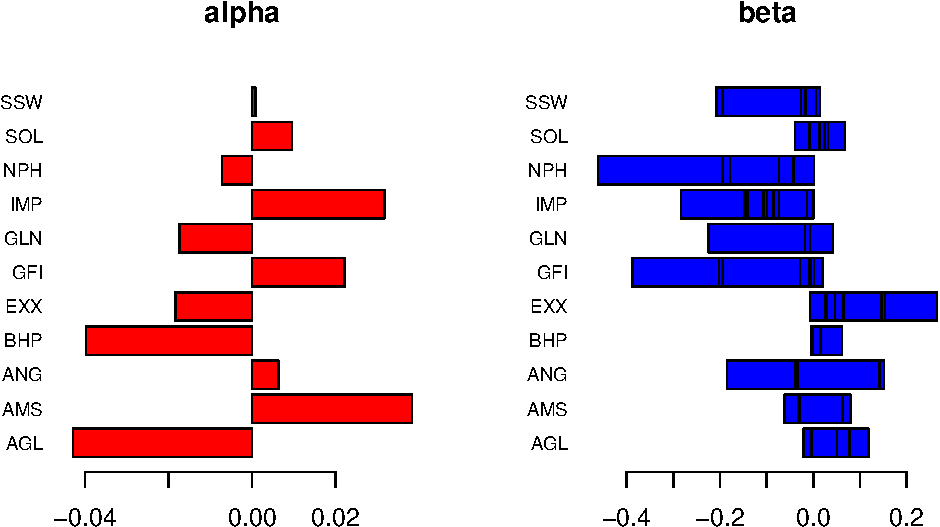
\includegraphics{Factor-Model_files/figure-latex/unnamed-chunk-14-1} \caption{Factor Analysis: Resources \label{Fig12}}\label{fig:unnamed-chunk-14}
\end{figure}

\hypertarget{discussion-of-results}{%
\subsection{\texorpdfstring{Discussion of Results
\label{Disc}}{Discussion of Results }}\label{discussion-of-results}}

\hypertarget{conclusion}{%
\section{Conclusion}\label{conclusion}}

\newpage

\hypertarget{references}{%
\section{References}\label{references}}

\hypertarget{refs}{}
\begin{CSLReferences}{1}{0}
\leavevmode\hypertarget{ref-Chen1986}{}%
Chen, N.-F., Roll, R. \& Ross, S. 1986. Economic forces and the stock
market. \emph{The Journal of Business}. 59(3):383--403.

\leavevmode\hypertarget{ref-Connor}{}%
Connor, G. 1995. The three types of factor models: A comparison of their
explanatory power. \emph{Financial Analysts Journal}. 51:42--46.

\leavevmode\hypertarget{ref-FTSE}{}%
{``Factsheet (ZAR) FTSE/JSE top 40 index''}. n.d. {[}Online{]},
Available:
\url{https://research.ftserussell.com/Analytics/Factsheets/Home/DownloadSingleIssue?issueName=J200\&amp;IsManual=false}.

\leavevmode\hypertarget{ref-Fama1992}{}%
Fama, E.F. \& French, K.R. 1992. {The Cross-Section of Expected Stock
Returns}. \emph{Journal of Finance}. 47(2):427--465.

\leavevmode\hypertarget{ref-Kim1987}{}%
Kim, M.K. \& Wu, C. 1987. {Macro-Economic Factors And Stock Returns}.
\emph{Journal of Financial Research}. 10(2):87--98.

\leavevmode\hypertarget{ref-Sharpe1964}{}%
Sharpe, W. 1964. Capital asset prices: A theory of market equilibrium
under conditions of risk. \emph{Journal of Finance}. 19(3):425--442.

\end{CSLReferences}

\newpage

\hypertarget{appendix-supplementary-tables}{%
\section{Appendix: Supplementary
Tables}\label{appendix-supplementary-tables}}

\hypertarget{financial}{%
\subsection{Financial}\label{financial}}

\begin{table}[H]

\caption{\label{tab:Beta_F}Factor Beta's: Financial}
\centering
\begin{tabular}[t]{l|l|l|l|l|l|l|l|l}
\hline
  & US\_10Yr & Bcom\_Index & VIX & USDZAR & MM.Rate & Real.GDP & Real.INV & Inflation\\
\hline
ABG & -0.0133 & -0.0056 & 0.0306 & 0.0976 & 0.0133 & 0.1730 & -0.0981 & 0.0000\\
\hline
CPI & -0.0113 & 0.0554 & 0.0137 & 0.0435 & 0.0275 & 0.3649 & -0.1153 & -0.0192\\
\hline
DSY & -0.0011 & 0.0344 & 0.0168 & 0.1036 & 0.0003 & 0.1265 & -0.0930 & -0.0001\\
\hline
FSR & -0.0084 & 0.0091 & 0.0097 & 0.0494 & 0.0034 & -0.1884 & 0.0182 & 0.0034\\
\hline
GRT & -0.0063 & 0.0230 & 0.0164 & 0.0834 & 0.0047 & 0.1469 & -0.0032 & 0.0006\\
\hline
INL & -0.0017 & 0.0076 & 0.0077 & 0.0339 & 0.0088 & 0.0102 & -0.0150 & 0.0013\\
\hline
INP & -0.0026 & 0.0340 & 0.0083 & 0.0686 & 0.0051 & 0.1847 & -0.1322 & -0.0077\\
\hline
NED & -0.0117 & 0.0071 & 0.0245 & 0.0863 & 0.0086 & 0.1478 & -0.0415 & 0.0035\\
\hline
SBK & -0.0022 & -0.0311 & 0.0093 & 0.0319 & 0.0065 & -0.1362 & 0.1003 & 0.0023\\
\hline
SLM & -0.0061 & -0.0567 & 0.0035 & 0.0030 & -0.0116 & -0.0363 & 0.0530 & 0.0059\\
\hline
\end{tabular}
\end{table}

\begin{table}[H]

\caption{\label{tab:Alpha_F}Factor Alpha's: Financial}
\centering
\begin{tabular}[t]{l|l}
\hline
  & x\\
\hline
ABG & -0.0073\\
\hline
CPI & -0.0193\\
\hline
DSY & 0.0025\\
\hline
FSR & 0.0029\\
\hline
GRT & -0.0009\\
\hline
INL & -0.0151\\
\hline
INP & -0.0026\\
\hline
NED & -0.0045\\
\hline
SBK & -0.0123\\
\hline
SLM & 0.0286\\
\hline
\end{tabular}
\end{table}

\begin{table}[H]

\caption{\label{tab:Covariance Matrix_F}Covariance Matrix: Financial}
\centering
\begin{tabular}[t]{l|l|l|l|l|l|l|l|l|l|l}
\hline
  & ABG & CPI & DSY & FSR & GRT & INL & INP & NED & SBK & SLM\\
\hline
ABG & 9e-04 & 1e-04 & 1e-04 & 1e-04 & 1e-04 & 1e-04 & 1e-04 & 2e-04 & 1e-04 & 1e-04\\
\hline
CPI & 1e-04 & 5e-04 & 0e+00 & 0e+00 & 1e-04 & 0e+00 & 0e+00 & 1e-04 & 0e+00 & 0e+00\\
\hline
DSY & 1e-04 & 0e+00 & 4e-04 & 0e+00 & 1e-04 & 0e+00 & 0e+00 & 1e-04 & 0e+00 & 0e+00\\
\hline
FSR & 1e-04 & 0e+00 & 0e+00 & 5e-04 & 0e+00 & 0e+00 & 0e+00 & 1e-04 & 0e+00 & 0e+00\\
\hline
GRT & 1e-04 & 1e-04 & 1e-04 & 0e+00 & 4e-04 & 0e+00 & 0e+00 & 1e-04 & 1e-04 & 0e+00\\
\hline
INL & 1e-04 & 0e+00 & 0e+00 & 0e+00 & 0e+00 & 3e-04 & 0e+00 & 1e-04 & 0e+00 & 0e+00\\
\hline
INP & 1e-04 & 0e+00 & 0e+00 & 0e+00 & 0e+00 & 0e+00 & 4e-04 & 0e+00 & 0e+00 & 0e+00\\
\hline
NED & 2e-04 & 1e-04 & 1e-04 & 1e-04 & 1e-04 & 1e-04 & 0e+00 & 6e-04 & 1e-04 & 1e-04\\
\hline
SBK & 1e-04 & 0e+00 & 0e+00 & 0e+00 & 1e-04 & 0e+00 & 0e+00 & 1e-04 & 6e-04 & 0e+00\\
\hline
SLM & 1e-04 & 0e+00 & 0e+00 & 0e+00 & 0e+00 & 0e+00 & 0e+00 & 1e-04 & 0e+00 & 4e-04\\
\hline
\end{tabular}
\end{table}

\newpage

\hypertarget{industrial}{%
\subsection{Industrial}\label{industrial}}

\begin{table}[H]

\caption{\label{tab:Beta_I}Factor Beta's: Industrial}
\centering
\begin{tabular}[t]{l|l|l|l|l|l|l|l|l}
\hline
  & US\_10Yr & Bcom\_Index & VIX & USDZAR & MM.Rate & Real.GDP & Real.INV & Inflation\\
\hline
APN & 0.0005 & -0.0506 & 0.0028 & 0.0265 & 0.0018 & -0.0411 & 0.0063 & 0.0220\\
\hline
BID & 0.0001 & 0.0802 & 0.0059 & 0.0928 & 0.0088 & 0.1476 & -0.0809 & 0.0003\\
\hline
BTI & -0.0100 & 0.0125 & 0.0086 & 0.0274 & 0.0247 & 0.0569 & -0.0162 & -0.0127\\
\hline
BVT & -0.0087 & 0.0050 & 0.0150 & 0.0690 & 0.0030 & 0.0046 & 0.0404 & 0.0001\\
\hline
CFR & 0.0029 & -0.0017 & -0.0094 & 0.0403 & 0.0212 & 0.0651 & -0.0622 & -0.0011\\
\hline
CLS & -0.0029 & -0.0040 & 0.0004 & 0.0153 & 0.0116 & -0.0488 & 0.0009 & 0.0089\\
\hline
MNP & -0.0005 & 0.0083 & 0.0101 & 0.0532 & 0.0188 & -0.0453 & -0.0316 & 0.0002\\
\hline
MRP & 0.0069 & -0.0046 & 0.0045 & 0.0441 & -0.0104 & -0.2065 & 0.1566 & 0.0037\\
\hline
MTN & -0.0051 & -0.0701 & 0.0312 & 0.0190 & -0.0010 & 0.0230 & 0.0244 & 0.0001\\
\hline
NPN & 0.0005 & -0.0068 & -0.0086 & 0.0493 & 0.0081 & -0.0125 & -0.0537 & 0.0027\\
\hline
SHP & 0.0026 & -0.0013 & 0.0016 & 0.0038 & 0.0013 & -0.1616 & 0.1257 & -0.0009\\
\hline
SPP & 0.0048 & -0.0038 & 0.0081 & -0.0091 & 0.0023 & -0.1399 & 0.1479 & 0.0016\\
\hline
VOD & 0.0024 & -0.0065 & 0.0059 & -0.0181 & 0.0055 & -0.0323 & 0.0666 & -0.0075\\
\hline
WHL & 0.0082 & 0.0223 & 0.0030 & 0.0183 & 0.0042 & -0.2556 & 0.1899 & 0.0032\\
\hline
\end{tabular}
\end{table}

\begin{table}[H]

\caption{\label{tab:Alpha_I}Factor Alpha's: Industrial}
\centering
\begin{tabular}[t]{l|l}
\hline
  & x\\
\hline
APN & -0.0154\\
\hline
BID & -0.0169\\
\hline
BTI & -0.0263\\
\hline
BVT & 0.0087\\
\hline
CFR & -0.0469\\
\hline
CLS & -0.0246\\
\hline
MNP & -0.0339\\
\hline
MRP & 0.0128\\
\hline
MTN & 0.0098\\
\hline
NPN & -0.0137\\
\hline
SHP & -0.0016\\
\hline
SPP & -0.0059\\
\hline
VOD & -0.0069\\
\hline
WHL & -0.0160\\
\hline
\end{tabular}
\end{table}

\begin{table}[H]

\caption{\label{tab:Covariance Matrix_I}Covariance Matrix: Industrial}
\centering
\begin{tabular}[t]{l|l|l|l|l|l|l|l|l|l|l|l|l|l|l}
\hline
  & APN & BID & BTI & BVT & CFR & CLS & MNP & MRP & MTN & NPN & SHP & SPP & VOD & WHL\\
\hline
APN & 5e-04 & 0e+00 & 0e+00 & 1e-04 & 0e+00 & 0e+00 & 0e+00 & 0e+00 & 0.0001 & 0e+00 & 0e+00 & 0e+00 & 0e+00 & 0e+00\\
\hline
BID & 0e+00 & 5e-04 & 0e+00 & 0e+00 & 0e+00 & 0e+00 & 0e+00 & 0e+00 & 0.0000 & 0e+00 & 0e+00 & 0e+00 & 0e+00 & 0e+00\\
\hline
BTI & 0e+00 & 0e+00 & 2e-04 & 0e+00 & 0e+00 & 0e+00 & 0e+00 & 0e+00 & 0.0001 & 0e+00 & 0e+00 & 0e+00 & 0e+00 & 0e+00\\
\hline
BVT & 1e-04 & 0e+00 & 0e+00 & 4e-04 & 0e+00 & 0e+00 & 0e+00 & 0e+00 & 0.0001 & 0e+00 & 0e+00 & 0e+00 & 0e+00 & 0e+00\\
\hline
CFR & 0e+00 & 0e+00 & 0e+00 & 0e+00 & 3e-04 & 0e+00 & 0e+00 & 0e+00 & 0.0000 & 0e+00 & 0e+00 & 0e+00 & 0e+00 & 0e+00\\
\hline
CLS & 0e+00 & 0e+00 & 0e+00 & 0e+00 & 0e+00 & 5e-04 & 0e+00 & 0e+00 & 0.0000 & 0e+00 & 0e+00 & 0e+00 & 0e+00 & 0e+00\\
\hline
MNP & 0e+00 & 0e+00 & 0e+00 & 0e+00 & 0e+00 & 0e+00 & 3e-04 & 0e+00 & 0.0001 & 0e+00 & 0e+00 & 0e+00 & 0e+00 & 0e+00\\
\hline
MRP & 0e+00 & 0e+00 & 0e+00 & 0e+00 & 0e+00 & 0e+00 & 0e+00 & 4e-04 & 0.0001 & 0e+00 & 0e+00 & 0e+00 & 0e+00 & 0e+00\\
\hline
MTN & 1e-04 & 0e+00 & 1e-04 & 1e-04 & 0e+00 & 0e+00 & 1e-04 & 1e-04 & 0.0011 & 0e+00 & 0e+00 & 0e+00 & 0e+00 & 0e+00\\
\hline
NPN & 0e+00 & 0e+00 & 0e+00 & 0e+00 & 0e+00 & 0e+00 & 0e+00 & 0e+00 & 0.0000 & 4e-04 & 0e+00 & 0e+00 & 0e+00 & 0e+00\\
\hline
SHP & 0e+00 & 0e+00 & 0e+00 & 0e+00 & 0e+00 & 0e+00 & 0e+00 & 0e+00 & 0.0000 & 0e+00 & 3e-04 & 0e+00 & 0e+00 & 0e+00\\
\hline
SPP & 0e+00 & 0e+00 & 0e+00 & 0e+00 & 0e+00 & 0e+00 & 0e+00 & 0e+00 & 0.0000 & 0e+00 & 0e+00 & 2e-04 & 0e+00 & 0e+00\\
\hline
VOD & 0e+00 & 0e+00 & 0e+00 & 0e+00 & 0e+00 & 0e+00 & 0e+00 & 0e+00 & 0.0000 & 0e+00 & 0e+00 & 0e+00 & 2e-04 & 0e+00\\
\hline
WHL & 0e+00 & 0e+00 & 0e+00 & 0e+00 & 0e+00 & 0e+00 & 0e+00 & 0e+00 & 0.0000 & 0e+00 & 0e+00 & 0e+00 & 0e+00 & 3e-04\\
\hline
\end{tabular}
\end{table}

\newpage

\hypertarget{resources}{%
\subsection{Resources}\label{resources}}

\begin{table}[H]

\caption{\label{tab:Beta_R}Factor Beta's: Resources}
\centering
\begin{tabular}[t]{l|l|l|l|l|l|l|l|l}
\hline
  & US\_10Yr & Bcom\_Index & VIX & USDZAR & MM.Rate & Real.GDP & Real.INV & Inflation\\
\hline
AGL & -0.0206 & 0.0168 & -0.0002 & 0.0548 & 0.0347 & 0.0327 & -0.0416 & 0.0011\\
\hline
AMS & 0.0009 & 0.0040 & 0.0093 & 0.0655 & -0.0169 & -0.1244 & 0.0329 & -0.0044\\
\hline
ANG & 0.0158 & 0.0556 & 0.0015 & 0.0786 & -0.0093 & -0.3271 & 0.1507 & -0.0053\\
\hline
BHP & -0.0040 & 0.0021 & -0.0007 & 0.0409 & 0.0232 & -0.0461 & -0.0156 & -0.0022\\
\hline
EXX & -0.0074 & 0.0331 & 0.0033 & 0.0174 & 0.0187 & 0.1998 & -0.1114 & -0.0073\\
\hline
GFI & 0.0197 & -0.0179 & -0.0084 & -0.0029 & -0.0194 & -0.3582 & 0.1927 & -0.0074\\
\hline
GLN & -0.0068 & 0.0015 & 0.0193 & 0.0039 & 0.0320 & -0.2825 & 0.1495 & 0.0145\\
\hline
IMP & -0.0134 & -0.0604 & -0.0120 & -0.0134 & -0.0073 & -0.1765 & 0.1362 & 0.0055\\
\hline
NPH & 0.0016 & -0.0527 & 0.0093 & -0.0315 & 0.0003 & -0.3881 & 0.2661 & 0.0167\\
\hline
SOL & -0.0109 & -0.0287 & 0.0319 & 0.0201 & 0.0004 & 0.0549 & -0.0442 & 0.0076\\
\hline
SSW & 0.0214 & -0.0425 & -0.0038 & -0.0478 & -0.0094 & -0.2192 & 0.0661 & -0.0014\\
\hline
\end{tabular}
\end{table}

\begin{table}[H]

\caption{\label{tab:Alpha_R}Factor Alpha's: Resources}
\centering
\begin{tabular}[t]{l|l}
\hline
  & x\\
\hline
AGL & -0.0429\\
\hline
AMS & 0.0383\\
\hline
ANG & 0.0063\\
\hline
BHP & -0.0398\\
\hline
EXX & -0.0184\\
\hline
GFI & 0.0222\\
\hline
GLN & -0.0557\\
\hline
IMP & 0.0317\\
\hline
NPH & -0.0072\\
\hline
SOL & 0.0095\\
\hline
SSW & 0.0000\\
\hline
\end{tabular}
\end{table}

\begin{table}[H]

\caption{\label{tab:Covariance Matrix_R}Covariance Matrix: Resources}
\centering
\begin{tabular}[t]{l|l|l|l|l|l|l|l|l|l|l|l}
\hline
  & AGL & AMS & ANG & BHP & EXX & GFI & GLN & IMP & NPH & SOL & SSW\\
\hline
AGL & 4e-04 & 0e+00 & 0e+00 & 0e+00 & 0e+00 & 0e+00 & 0.0001 & 0e+00 & 0e+00 & 0e+00 & 0e+00\\
\hline
AMS & 0e+00 & 6e-04 & 0e+00 & 0e+00 & 0e+00 & 0e+00 & 0.0000 & 0e+00 & 0e+00 & 1e-04 & 0e+00\\
\hline
ANG & 0e+00 & 0e+00 & 5e-04 & 0e+00 & 0e+00 & 1e-04 & 0.0000 & 0e+00 & 0e+00 & 0e+00 & 0e+00\\
\hline
BHP & 0e+00 & 0e+00 & 0e+00 & 3e-04 & 0e+00 & 0e+00 & 0.0001 & 0e+00 & 0e+00 & 0e+00 & 0e+00\\
\hline
EXX & 0e+00 & 0e+00 & 0e+00 & 0e+00 & 5e-04 & 0e+00 & 0.0000 & 0e+00 & 0e+00 & 0e+00 & 0e+00\\
\hline
GFI & 0e+00 & 0e+00 & 1e-04 & 0e+00 & 0e+00 & 6e-04 & 0.0000 & 0e+00 & 0e+00 & -1e-04 & 1e-04\\
\hline
GLN & 1e-04 & 0e+00 & 0e+00 & 1e-04 & 0e+00 & 0e+00 & 0.0015 & 0e+00 & 1e-04 & 1e-04 & 0e+00\\
\hline
IMP & 0e+00 & 0e+00 & 0e+00 & 0e+00 & 0e+00 & 0e+00 & 0.0000 & 6e-04 & 0e+00 & 0e+00 & 0e+00\\
\hline
NPH & 0e+00 & 0e+00 & 0e+00 & 0e+00 & 0e+00 & 0e+00 & 0.0001 & 0e+00 & 8e-04 & 1e-04 & 0e+00\\
\hline
SOL & 0e+00 & 1e-04 & 0e+00 & 0e+00 & 0e+00 & -1e-04 & 0.0001 & 0e+00 & 1e-04 & 7e-04 & 0e+00\\
\hline
SSW & 0e+00 & 0e+00 & 0e+00 & 0e+00 & 0e+00 & 1e-04 & 0.0000 & 0e+00 & 0e+00 & 0e+00 & 7e-04\\
\hline
\end{tabular}
\end{table}

\bibliography{Tex/ref}





\end{document}
